% set 0.5 inch indentation
\setlength{\parindent}{0in}
% set paragraph space = 0 space
\setlength{\parskip}{1.5mm}
% set line space 1.5
\setlength{\baselineskip}{1.6em}

\chapter{INTRODUCTION}
\section{Background}
Masked Language Modeling (MLM) is key task for training vision-language (VL) models\cite{albef, mplug, uniter, beit-3}.
Most work randomly masked some word token to a fixed percentage in the training process, while expected model to predict the missing token based on vision modal.
\citeA{mask_object, selective_masking} suggest that by masking specific words in the training process often yield better performance.


However, 


\begin{figure}[h]
    \caption{Overall methodology}
    \label{fig:overall_method}
    Self-distillation training with image text joined representation.
    \begin{center}
        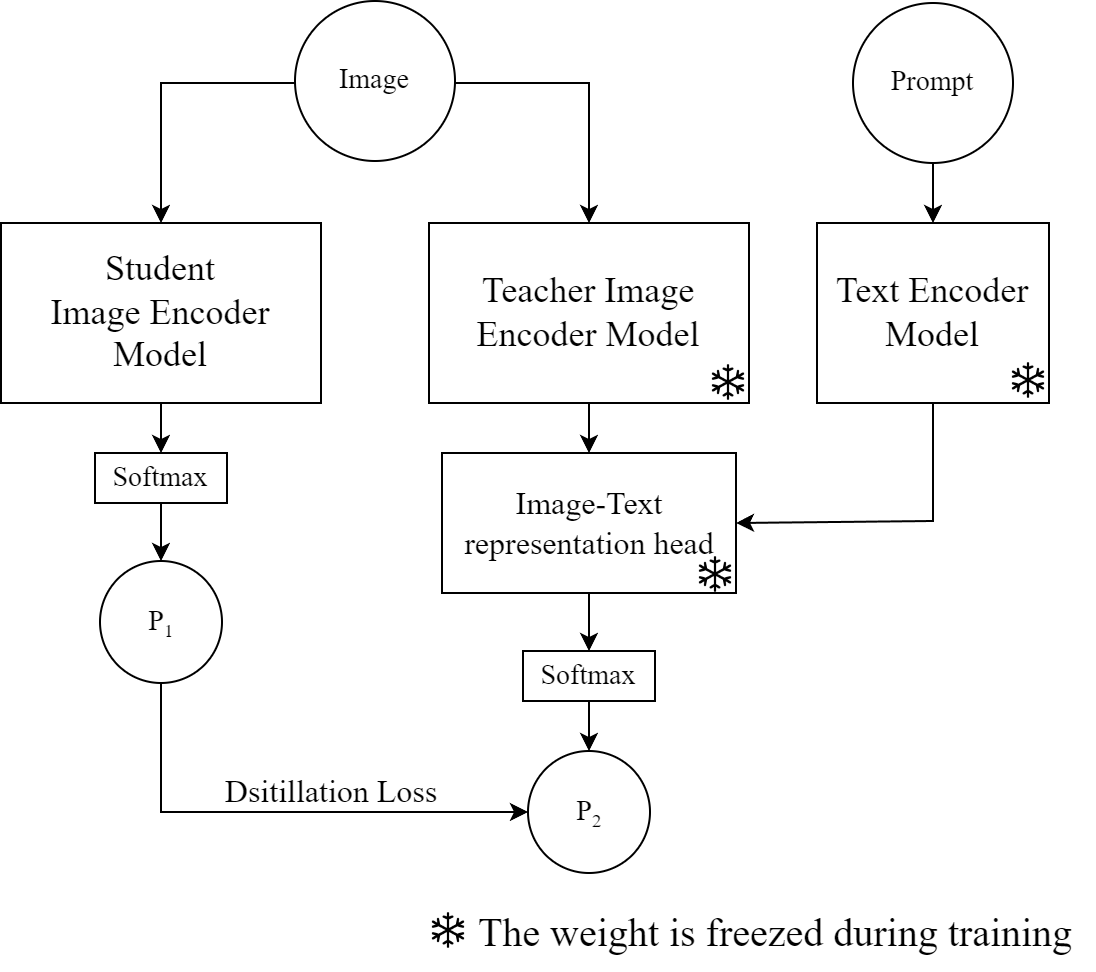
\includegraphics[width=0.75\textwidth]{Images/OverviewMethod.png}
    \end{center}
    \small
\end{figure}
